\frame{
\frametitle{Introduction: Model-Constrained Machine Learning Approach}

\vspace{5ex}

\resizebox{1\textwidth}{!}{
    
\tikzset{every picture/.style={line width=0.75pt}} %set default line width to 0.75pt        

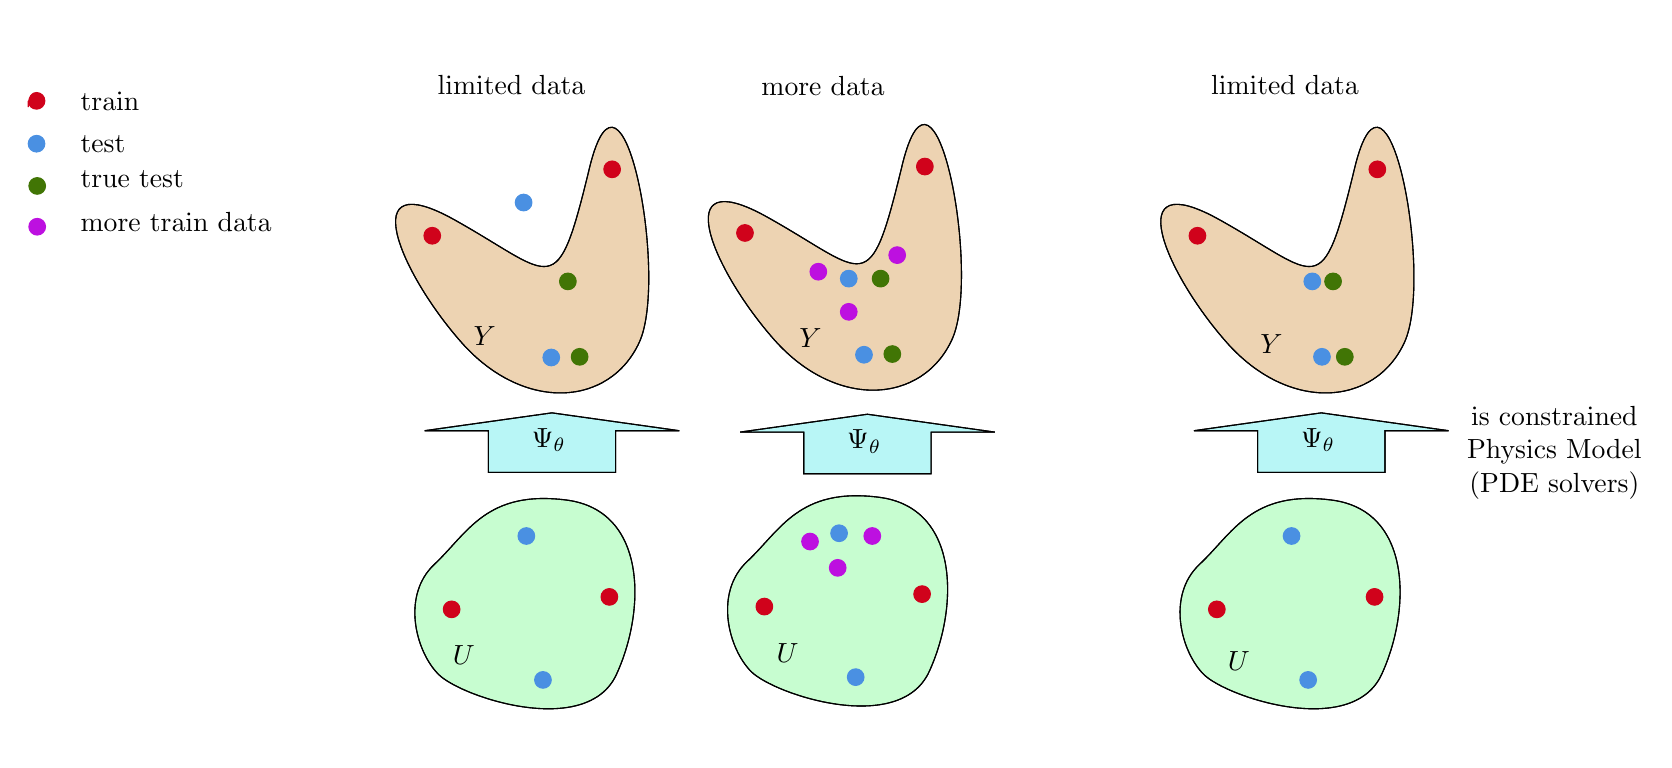
\begin{tikzpicture}[x=0.75pt,y=0.75pt,yscale=-1,xscale=1]
%uncomment if require: \path (0,500); %set diagram left start at 0, and has height of 500

%Shape: Polygon Curved [id:ds09447833398141592] 
\draw  [fill={rgb, 255:red, 197; green, 110; blue, 0 }  ,fill opacity=.3 ] (54.67,193) .. controls (24.67,159) and (3.15,107.04) .. (51.41,134.02) .. controls (99.67,161) and (100.41,175.02) .. (116.41,109.02) .. controls (132.41,43.02) and (154.67,162) .. (140.41,193.02) .. controls (126.15,224.04) and (84.67,227) .. (54.67,193) -- cycle ;
%Shape: Polygon Curved [id:ds8342971788940445] 
\draw  [fill={rgb, 255:red, 70; green, 248; blue, 100 }  ,fill opacity=.3 ] (43.67,353) .. controls (32.67,342) and (25.67,315) .. (41.67,300) .. controls (57.67,285) and (66.67,264) .. (105.41,269.02) .. controls (144.15,274.04) and (143.67,322) .. (129.41,353.02) .. controls (115.15,384.04) and (54.67,364) .. (43.67,353) -- cycle ;
%Shape: Polygon Curved [id:ds3279137678612456] 
\draw  [fill={rgb, 255:red, 197; green, 110; blue, 0 }  ,fill opacity=.3 ] (205.33,191.67) .. controls (175.33,157.67) and (153.82,105.7) .. (202.07,132.69) .. controls (250.33,159.67) and (251.07,173.69) .. (267.07,107.69) .. controls (283.07,41.69) and (305.33,160.67) .. (291.07,191.69) .. controls (276.82,222.7) and (235.33,225.67) .. (205.33,191.67) -- cycle ;
%Shape: Polygon Curved [id:ds20441696774386264] 
\draw  [fill={rgb, 255:red, 70; green, 248; blue, 100 }  ,fill opacity=.3 ] (194.33,351.67) .. controls (183.33,340.67) and (176.33,313.67) .. (192.33,298.67) .. controls (208.33,283.67) and (217.33,262.67) .. (256.07,267.69) .. controls (294.82,272.7) and (294.33,320.67) .. (280.07,351.69) .. controls (265.82,382.7) and (205.33,362.67) .. (194.33,351.67) -- cycle ;
%Shape: Polygon Curved [id:ds07726784585526025] 
\draw  [fill={rgb, 255:red, 197; green, 110; blue, 0 }  ,fill opacity=.3 ] (423.33,193) .. controls (393.33,159) and (371.82,107.04) .. (420.07,134.02) .. controls (468.33,161) and (469.07,175.02) .. (485.07,109.02) .. controls (501.07,43.02) and (523.33,162) .. (509.07,193.02) .. controls (494.82,224.04) and (453.33,227) .. (423.33,193) -- cycle ;
%Shape: Polygon Curved [id:ds010660115400260906] 
\draw  [fill={rgb, 255:red, 70; green, 248; blue, 100 }  ,fill opacity=.3 ] (412.33,353) .. controls (401.33,342) and (394.33,315) .. (410.33,300) .. controls (426.33,285) and (435.33,264) .. (474.07,269.02) .. controls (512.82,274.04) and (512.33,322) .. (498.07,353.02) .. controls (483.82,384.04) and (423.33,364) .. (412.33,353) -- cycle ;
%Up Arrow [id:dp6794269498576513] 
\draw  [fill={rgb, 255:red, 20; green, 225; blue, 225 }  ,fill opacity=.3 ] (37,235.6) -- (98.33,227) -- (159.67,235.6) -- (129,235.6) -- (129,255.67) -- (67.67,255.67) -- (67.67,235.6) -- cycle ;
%Up Arrow [id:dp09726735914616291] 
\draw  [fill={rgb, 255:red, 20; green, 225; blue, 225 }  ,fill opacity=.3 ] (189,236.27) -- (250.33,227.67) -- (311.67,236.27) -- (281,236.27) -- (281,256.33) -- (219.67,256.33) -- (219.67,236.27) -- cycle ;
%Up Arrow [id:dp5149313118072518] 
\draw  [fill={rgb, 255:red, 20; green, 225; blue, 225 }  ,fill opacity=.3 ] (407.67,235.6) -- (469,227) -- (530.33,235.6) -- (499.67,235.6) -- (499.67,255.67) -- (438.33,255.67) -- (438.33,235.6) -- cycle ;

%Shape: Polygon Curved [id:ds09447833398141592] 
\draw   (54.67,193) .. controls (24.67,159) and (3.15,107.04) .. (51.41,134.02) .. controls (99.67,161) and (100.41,175.02) .. (116.41,109.02) .. controls (132.41,43.02) and (154.67,162) .. (140.41,193.02) .. controls (126.15,224.04) and (84.67,227) .. (54.67,193) -- cycle ;
%Shape: Polygon Curved [id:ds8342971788940445] 
\draw   (43.67,353) .. controls (32.67,342) and (25.67,315) .. (41.67,300) .. controls (57.67,285) and (66.67,264) .. (105.41,269.02) .. controls (144.15,274.04) and (143.67,322) .. (129.41,353.02) .. controls (115.15,384.04) and (54.67,364) .. (43.67,353) -- cycle ;
%Shape: Circle [id:dp26432558400430295] 
\draw  [color={rgb, 255:red, 208; green, 2; blue, 27 }  ,draw opacity=1 ][fill={rgb, 255:red, 208; green, 2; blue, 27 }  ,fill opacity=1 ] (46,321.67) .. controls (46,319.46) and (47.79,317.67) .. (50,317.67) .. controls (52.21,317.67) and (54,319.46) .. (54,321.67) .. controls (54,323.88) and (52.21,325.67) .. (50,325.67) .. controls (47.79,325.67) and (46,323.88) .. (46,321.67) -- cycle ;
%Shape: Circle [id:dp7486480801214225] 
\draw  [color={rgb, 255:red, 208; green, 2; blue, 27 }  ,draw opacity=1 ][fill={rgb, 255:red, 208; green, 2; blue, 27 }  ,fill opacity=1 ] (122,315.67) .. controls (122,313.46) and (123.79,311.67) .. (126,311.67) .. controls (128.21,311.67) and (130,313.46) .. (130,315.67) .. controls (130,317.88) and (128.21,319.67) .. (126,319.67) .. controls (123.79,319.67) and (122,317.88) .. (122,315.67) -- cycle ;
%Shape: Circle [id:dp9817597880379183] 
\draw  [color={rgb, 255:red, 208; green, 2; blue, 27 }  ,draw opacity=1 ][fill={rgb, 255:red, 208; green, 2; blue, 27 }  ,fill opacity=1 ] (36.67,141.67) .. controls (36.67,139.46) and (38.46,137.67) .. (40.67,137.67) .. controls (42.88,137.67) and (44.67,139.46) .. (44.67,141.67) .. controls (44.67,143.88) and (42.88,145.67) .. (40.67,145.67) .. controls (38.46,145.67) and (36.67,143.88) .. (36.67,141.67) -- cycle ;
%Shape: Circle [id:dp006804475688651168] 
\draw  [color={rgb, 255:red, 208; green, 2; blue, 27 }  ,draw opacity=1 ][fill={rgb, 255:red, 208; green, 2; blue, 27 }  ,fill opacity=1 ] (123.33,109.67) .. controls (123.33,107.46) and (125.12,105.67) .. (127.33,105.67) .. controls (129.54,105.67) and (131.33,107.46) .. (131.33,109.67) .. controls (131.33,111.88) and (129.54,113.67) .. (127.33,113.67) .. controls (125.12,113.67) and (123.33,111.88) .. (123.33,109.67) -- cycle ;
%Shape: Circle [id:dp009892328190684307] 
\draw  [color={rgb, 255:red, 74; green, 144; blue, 226 }  ,draw opacity=1 ][fill={rgb, 255:red, 74; green, 144; blue, 226 }  ,fill opacity=1 ] (90,355.67) .. controls (90,353.46) and (91.79,351.67) .. (94,351.67) .. controls (96.21,351.67) and (98,353.46) .. (98,355.67) .. controls (98,357.88) and (96.21,359.67) .. (94,359.67) .. controls (91.79,359.67) and (90,357.88) .. (90,355.67) -- cycle ;
%Shape: Circle [id:dp3982721887803482] 
\draw  [color={rgb, 255:red, 74; green, 144; blue, 226 }  ,draw opacity=1 ][fill={rgb, 255:red, 74; green, 144; blue, 226 }  ,fill opacity=1 ] (82,286.33) .. controls (82,284.12) and (83.79,282.33) .. (86,282.33) .. controls (88.21,282.33) and (90,284.12) .. (90,286.33) .. controls (90,288.54) and (88.21,290.33) .. (86,290.33) .. controls (83.79,290.33) and (82,288.54) .. (82,286.33) -- cycle ;
%Shape: Circle [id:dp49175636396347844] 
\draw  [color={rgb, 255:red, 74; green, 144; blue, 226 }  ,draw opacity=1 ][fill={rgb, 255:red, 74; green, 144; blue, 226 }  ,fill opacity=1 ] (94,200.33) .. controls (94,198.12) and (95.79,196.33) .. (98,196.33) .. controls (100.21,196.33) and (102,198.12) .. (102,200.33) .. controls (102,202.54) and (100.21,204.33) .. (98,204.33) .. controls (95.79,204.33) and (94,202.54) .. (94,200.33) -- cycle ;
%Shape: Circle [id:dp21682181561205804] 
\draw  [color={rgb, 255:red, 74; green, 144; blue, 226 }  ,draw opacity=1 ][fill={rgb, 255:red, 74; green, 144; blue, 226 }  ,fill opacity=1 ] (80.67,125.67) .. controls (80.67,123.46) and (82.46,121.67) .. (84.67,121.67) .. controls (86.88,121.67) and (88.67,123.46) .. (88.67,125.67) .. controls (88.67,127.88) and (86.88,129.67) .. (84.67,129.67) .. controls (82.46,129.67) and (80.67,127.88) .. (80.67,125.67) -- cycle ;
%Shape: Circle [id:dp8907831670398318] 
\draw  [color={rgb, 255:red, 65; green, 117; blue, 5 }  ,draw opacity=1 ][fill={rgb, 255:red, 65; green, 117; blue, 5 }  ,fill opacity=1 ] (107.67,200) .. controls (107.67,197.79) and (109.46,196) .. (111.67,196) .. controls (113.88,196) and (115.67,197.79) .. (115.67,200) .. controls (115.67,202.21) and (113.88,204) .. (111.67,204) .. controls (109.46,204) and (107.67,202.21) .. (107.67,200) -- cycle ;
%Shape: Circle [id:dp5286507300103176] 
\draw  [color={rgb, 255:red, 65; green, 117; blue, 5 }  ,draw opacity=1 ][fill={rgb, 255:red, 65; green, 117; blue, 5 }  ,fill opacity=1 ] (102,163.67) .. controls (102,161.46) and (103.79,159.67) .. (106,159.67) .. controls (108.21,159.67) and (110,161.46) .. (110,163.67) .. controls (110,165.88) and (108.21,167.67) .. (106,167.67) .. controls (103.79,167.67) and (102,165.88) .. (102,163.67) -- cycle ;
%Shape: Polygon Curved [id:ds3279137678612456] 
\draw   (205.33,191.67) .. controls (175.33,157.67) and (153.82,105.7) .. (202.07,132.69) .. controls (250.33,159.67) and (251.07,173.69) .. (267.07,107.69) .. controls (283.07,41.69) and (305.33,160.67) .. (291.07,191.69) .. controls (276.82,222.7) and (235.33,225.67) .. (205.33,191.67) -- cycle ;
%Shape: Polygon Curved [id:ds20441696774386264] 
\draw   (194.33,351.67) .. controls (183.33,340.67) and (176.33,313.67) .. (192.33,298.67) .. controls (208.33,283.67) and (217.33,262.67) .. (256.07,267.69) .. controls (294.82,272.7) and (294.33,320.67) .. (280.07,351.69) .. controls (265.82,382.7) and (205.33,362.67) .. (194.33,351.67) -- cycle ;
%Shape: Circle [id:dp8376942440901165] 
\draw  [color={rgb, 255:red, 208; green, 2; blue, 27 }  ,draw opacity=1 ][fill={rgb, 255:red, 208; green, 2; blue, 27 }  ,fill opacity=1 ] (196.67,320.33) .. controls (196.67,318.12) and (198.46,316.33) .. (200.67,316.33) .. controls (202.88,316.33) and (204.67,318.12) .. (204.67,320.33) .. controls (204.67,322.54) and (202.88,324.33) .. (200.67,324.33) .. controls (198.46,324.33) and (196.67,322.54) .. (196.67,320.33) -- cycle ;
%Shape: Circle [id:dp6923958625920651] 
\draw  [color={rgb, 255:red, 208; green, 2; blue, 27 }  ,draw opacity=1 ][fill={rgb, 255:red, 208; green, 2; blue, 27 }  ,fill opacity=1 ] (272.67,314.33) .. controls (272.67,312.12) and (274.46,310.33) .. (276.67,310.33) .. controls (278.88,310.33) and (280.67,312.12) .. (280.67,314.33) .. controls (280.67,316.54) and (278.88,318.33) .. (276.67,318.33) .. controls (274.46,318.33) and (272.67,316.54) .. (272.67,314.33) -- cycle ;
%Shape: Circle [id:dp7389445208598843] 
\draw  [color={rgb, 255:red, 208; green, 2; blue, 27 }  ,draw opacity=1 ][fill={rgb, 255:red, 208; green, 2; blue, 27 }  ,fill opacity=1 ] (187.33,140.33) .. controls (187.33,138.12) and (189.12,136.33) .. (191.33,136.33) .. controls (193.54,136.33) and (195.33,138.12) .. (195.33,140.33) .. controls (195.33,142.54) and (193.54,144.33) .. (191.33,144.33) .. controls (189.12,144.33) and (187.33,142.54) .. (187.33,140.33) -- cycle ;
%Shape: Circle [id:dp09462367026507623] 
\draw  [color={rgb, 255:red, 208; green, 2; blue, 27 }  ,draw opacity=1 ][fill={rgb, 255:red, 208; green, 2; blue, 27 }  ,fill opacity=1 ] (274,108.33) .. controls (274,106.12) and (275.79,104.33) .. (278,104.33) .. controls (280.21,104.33) and (282,106.12) .. (282,108.33) .. controls (282,110.54) and (280.21,112.33) .. (278,112.33) .. controls (275.79,112.33) and (274,110.54) .. (274,108.33) -- cycle ;
%Shape: Circle [id:dp11319586275056814] 
\draw  [color={rgb, 255:red, 74; green, 144; blue, 226 }  ,draw opacity=1 ][fill={rgb, 255:red, 74; green, 144; blue, 226 }  ,fill opacity=1 ] (240.67,354.33) .. controls (240.67,352.12) and (242.46,350.33) .. (244.67,350.33) .. controls (246.88,350.33) and (248.67,352.12) .. (248.67,354.33) .. controls (248.67,356.54) and (246.88,358.33) .. (244.67,358.33) .. controls (242.46,358.33) and (240.67,356.54) .. (240.67,354.33) -- cycle ;
%Shape: Circle [id:dp8920361474219186] 
\draw  [color={rgb, 255:red, 74; green, 144; blue, 226 }  ,draw opacity=1 ][fill={rgb, 255:red, 74; green, 144; blue, 226 }  ,fill opacity=1 ] (232.67,285) .. controls (232.67,282.79) and (234.46,281) .. (236.67,281) .. controls (238.88,281) and (240.67,282.79) .. (240.67,285) .. controls (240.67,287.21) and (238.88,289) .. (236.67,289) .. controls (234.46,289) and (232.67,287.21) .. (232.67,285) -- cycle ;
%Shape: Circle [id:dp9966673763530642] 
\draw  [color={rgb, 255:red, 74; green, 144; blue, 226 }  ,draw opacity=1 ][fill={rgb, 255:red, 74; green, 144; blue, 226 }  ,fill opacity=1 ] (244.67,199) .. controls (244.67,196.79) and (246.46,195) .. (248.67,195) .. controls (250.88,195) and (252.67,196.79) .. (252.67,199) .. controls (252.67,201.21) and (250.88,203) .. (248.67,203) .. controls (246.46,203) and (244.67,201.21) .. (244.67,199) -- cycle ;
%Shape: Circle [id:dp3136076301608942] 
\draw  [color={rgb, 255:red, 74; green, 144; blue, 226 }  ,draw opacity=1 ][fill={rgb, 255:red, 74; green, 144; blue, 226 }  ,fill opacity=1 ] (237.33,162.33) .. controls (237.33,160.12) and (239.12,158.33) .. (241.33,158.33) .. controls (243.54,158.33) and (245.33,160.12) .. (245.33,162.33) .. controls (245.33,164.54) and (243.54,166.33) .. (241.33,166.33) .. controls (239.12,166.33) and (237.33,164.54) .. (237.33,162.33) -- cycle ;
%Shape: Circle [id:dp3648098032954873] 
\draw  [color={rgb, 255:red, 65; green, 117; blue, 5 }  ,draw opacity=1 ][fill={rgb, 255:red, 65; green, 117; blue, 5 }  ,fill opacity=1 ] (258.33,198.67) .. controls (258.33,196.46) and (260.12,194.67) .. (262.33,194.67) .. controls (264.54,194.67) and (266.33,196.46) .. (266.33,198.67) .. controls (266.33,200.88) and (264.54,202.67) .. (262.33,202.67) .. controls (260.12,202.67) and (258.33,200.88) .. (258.33,198.67) -- cycle ;
%Shape: Circle [id:dp512662669745621] 
\draw  [color={rgb, 255:red, 65; green, 117; blue, 5 }  ,draw opacity=1 ][fill={rgb, 255:red, 65; green, 117; blue, 5 }  ,fill opacity=1 ] (252.67,162.33) .. controls (252.67,160.12) and (254.46,158.33) .. (256.67,158.33) .. controls (258.88,158.33) and (260.67,160.12) .. (260.67,162.33) .. controls (260.67,164.54) and (258.88,166.33) .. (256.67,166.33) .. controls (254.46,166.33) and (252.67,164.54) .. (252.67,162.33) -- cycle ;
%Shape: Circle [id:dp5844049985343532] 
\draw  [color={rgb, 255:red, 189; green, 16; blue, 224 }  ,draw opacity=1 ][fill={rgb, 255:red, 189; green, 16; blue, 224 }  ,fill opacity=1 ] (218.67,289) .. controls (218.67,286.79) and (220.46,285) .. (222.67,285) .. controls (224.88,285) and (226.67,286.79) .. (226.67,289) .. controls (226.67,291.21) and (224.88,293) .. (222.67,293) .. controls (220.46,293) and (218.67,291.21) .. (218.67,289) -- cycle ;
%Shape: Circle [id:dp21392691792594376] 
\draw  [color={rgb, 255:red, 189; green, 16; blue, 224 }  ,draw opacity=1 ][fill={rgb, 255:red, 189; green, 16; blue, 224 }  ,fill opacity=1 ] (248.67,286.33) .. controls (248.67,284.12) and (250.46,282.33) .. (252.67,282.33) .. controls (254.88,282.33) and (256.67,284.12) .. (256.67,286.33) .. controls (256.67,288.54) and (254.88,290.33) .. (252.67,290.33) .. controls (250.46,290.33) and (248.67,288.54) .. (248.67,286.33) -- cycle ;
%Shape: Circle [id:dp03765555278678889] 
\draw  [color={rgb, 255:red, 189; green, 16; blue, 224 }  ,draw opacity=1 ][fill={rgb, 255:red, 189; green, 16; blue, 224 }  ,fill opacity=1 ] (222.67,159) .. controls (222.67,156.79) and (224.46,155) .. (226.67,155) .. controls (228.88,155) and (230.67,156.79) .. (230.67,159) .. controls (230.67,161.21) and (228.88,163) .. (226.67,163) .. controls (224.46,163) and (222.67,161.21) .. (222.67,159) -- cycle ;
%Shape: Circle [id:dp3713963754985672] 
\draw  [color={rgb, 255:red, 189; green, 16; blue, 224 }  ,draw opacity=1 ][fill={rgb, 255:red, 189; green, 16; blue, 224 }  ,fill opacity=1 ] (260.67,151) .. controls (260.67,148.79) and (262.46,147) .. (264.67,147) .. controls (266.88,147) and (268.67,148.79) .. (268.67,151) .. controls (268.67,153.21) and (266.88,155) .. (264.67,155) .. controls (262.46,155) and (260.67,153.21) .. (260.67,151) -- cycle ;
%Shape: Circle [id:dp4867530767856524] 
\draw  [color={rgb, 255:red, 189; green, 16; blue, 224 }  ,draw opacity=1 ][fill={rgb, 255:red, 189; green, 16; blue, 224 }  ,fill opacity=1 ] (232,301.67) .. controls (232,299.46) and (233.79,297.67) .. (236,297.67) .. controls (238.21,297.67) and (240,299.46) .. (240,301.67) .. controls (240,303.88) and (238.21,305.67) .. (236,305.67) .. controls (233.79,305.67) and (232,303.88) .. (232,301.67) -- cycle ;
%Shape: Circle [id:dp26156864275097613] 
\draw  [color={rgb, 255:red, 189; green, 16; blue, 224 }  ,draw opacity=1 ][fill={rgb, 255:red, 189; green, 16; blue, 224 }  ,fill opacity=1 ] (237.33,178.33) .. controls (237.33,176.12) and (239.12,174.33) .. (241.33,174.33) .. controls (243.54,174.33) and (245.33,176.12) .. (245.33,178.33) .. controls (245.33,180.54) and (243.54,182.33) .. (241.33,182.33) .. controls (239.12,182.33) and (237.33,180.54) .. (237.33,178.33) -- cycle ;
%Shape: Polygon Curved [id:ds07726784585526025] 
\draw   (423.33,193) .. controls (393.33,159) and (371.82,107.04) .. (420.07,134.02) .. controls (468.33,161) and (469.07,175.02) .. (485.07,109.02) .. controls (501.07,43.02) and (523.33,162) .. (509.07,193.02) .. controls (494.82,224.04) and (453.33,227) .. (423.33,193) -- cycle ;
%Shape: Polygon Curved [id:ds010660115400260906] 
\draw   (412.33,353) .. controls (401.33,342) and (394.33,315) .. (410.33,300) .. controls (426.33,285) and (435.33,264) .. (474.07,269.02) .. controls (512.82,274.04) and (512.33,322) .. (498.07,353.02) .. controls (483.82,384.04) and (423.33,364) .. (412.33,353) -- cycle ;
%Shape: Circle [id:dp6050150972945199] 
\draw  [color={rgb, 255:red, 208; green, 2; blue, 27 }  ,draw opacity=1 ][fill={rgb, 255:red, 208; green, 2; blue, 27 }  ,fill opacity=1 ] (414.67,321.67) .. controls (414.67,319.46) and (416.46,317.67) .. (418.67,317.67) .. controls (420.88,317.67) and (422.67,319.46) .. (422.67,321.67) .. controls (422.67,323.88) and (420.88,325.67) .. (418.67,325.67) .. controls (416.46,325.67) and (414.67,323.88) .. (414.67,321.67) -- cycle ;
%Shape: Circle [id:dp9364297613608107] 
\draw  [color={rgb, 255:red, 208; green, 2; blue, 27 }  ,draw opacity=1 ][fill={rgb, 255:red, 208; green, 2; blue, 27 }  ,fill opacity=1 ] (490.67,315.67) .. controls (490.67,313.46) and (492.46,311.67) .. (494.67,311.67) .. controls (496.88,311.67) and (498.67,313.46) .. (498.67,315.67) .. controls (498.67,317.88) and (496.88,319.67) .. (494.67,319.67) .. controls (492.46,319.67) and (490.67,317.88) .. (490.67,315.67) -- cycle ;
%Shape: Circle [id:dp23887389693118888] 
\draw  [color={rgb, 255:red, 208; green, 2; blue, 27 }  ,draw opacity=1 ][fill={rgb, 255:red, 208; green, 2; blue, 27 }  ,fill opacity=1 ] (405.33,141.67) .. controls (405.33,139.46) and (407.12,137.67) .. (409.33,137.67) .. controls (411.54,137.67) and (413.33,139.46) .. (413.33,141.67) .. controls (413.33,143.88) and (411.54,145.67) .. (409.33,145.67) .. controls (407.12,145.67) and (405.33,143.88) .. (405.33,141.67) -- cycle ;
%Shape: Circle [id:dp6245898218338471] 
\draw  [color={rgb, 255:red, 208; green, 2; blue, 27 }  ,draw opacity=1 ][fill={rgb, 255:red, 208; green, 2; blue, 27 }  ,fill opacity=1 ] (492,109.67) .. controls (492,107.46) and (493.79,105.67) .. (496,105.67) .. controls (498.21,105.67) and (500,107.46) .. (500,109.67) .. controls (500,111.88) and (498.21,113.67) .. (496,113.67) .. controls (493.79,113.67) and (492,111.88) .. (492,109.67) -- cycle ;
%Shape: Circle [id:dp9009813115521121] 
\draw  [color={rgb, 255:red, 74; green, 144; blue, 226 }  ,draw opacity=1 ][fill={rgb, 255:red, 74; green, 144; blue, 226 }  ,fill opacity=1 ] (458.67,355.67) .. controls (458.67,353.46) and (460.46,351.67) .. (462.67,351.67) .. controls (464.88,351.67) and (466.67,353.46) .. (466.67,355.67) .. controls (466.67,357.88) and (464.88,359.67) .. (462.67,359.67) .. controls (460.46,359.67) and (458.67,357.88) .. (458.67,355.67) -- cycle ;
%Shape: Circle [id:dp5708756535513383] 
\draw  [color={rgb, 255:red, 74; green, 144; blue, 226 }  ,draw opacity=1 ][fill={rgb, 255:red, 74; green, 144; blue, 226 }  ,fill opacity=1 ] (450.67,286.33) .. controls (450.67,284.12) and (452.46,282.33) .. (454.67,282.33) .. controls (456.88,282.33) and (458.67,284.12) .. (458.67,286.33) .. controls (458.67,288.54) and (456.88,290.33) .. (454.67,290.33) .. controls (452.46,290.33) and (450.67,288.54) .. (450.67,286.33) -- cycle ;
%Shape: Circle [id:dp5227952073213964] 
\draw  [color={rgb, 255:red, 74; green, 144; blue, 226 }  ,draw opacity=1 ][fill={rgb, 255:red, 74; green, 144; blue, 226 }  ,fill opacity=1 ] (465.33,200) .. controls (465.33,197.79) and (467.12,196) .. (469.33,196) .. controls (471.54,196) and (473.33,197.79) .. (473.33,200) .. controls (473.33,202.21) and (471.54,204) .. (469.33,204) .. controls (467.12,204) and (465.33,202.21) .. (465.33,200) -- cycle ;
%Shape: Circle [id:dp8422423939560267] 
\draw  [color={rgb, 255:red, 74; green, 144; blue, 226 }  ,draw opacity=1 ][fill={rgb, 255:red, 74; green, 144; blue, 226 }  ,fill opacity=1 ] (460.67,163.67) .. controls (460.67,161.46) and (462.46,159.67) .. (464.67,159.67) .. controls (466.88,159.67) and (468.67,161.46) .. (468.67,163.67) .. controls (468.67,165.88) and (466.88,167.67) .. (464.67,167.67) .. controls (462.46,167.67) and (460.67,165.88) .. (460.67,163.67) -- cycle ;
%Shape: Circle [id:dp3798294341721118] 
\draw  [color={rgb, 255:red, 65; green, 117; blue, 5 }  ,draw opacity=1 ][fill={rgb, 255:red, 65; green, 117; blue, 5 }  ,fill opacity=1 ] (476.33,200) .. controls (476.33,197.79) and (478.12,196) .. (480.33,196) .. controls (482.54,196) and (484.33,197.79) .. (484.33,200) .. controls (484.33,202.21) and (482.54,204) .. (480.33,204) .. controls (478.12,204) and (476.33,202.21) .. (476.33,200) -- cycle ;
%Shape: Circle [id:dp8266340050542115] 
\draw  [color={rgb, 255:red, 65; green, 117; blue, 5 }  ,draw opacity=1 ][fill={rgb, 255:red, 65; green, 117; blue, 5 }  ,fill opacity=1 ] (470.67,163.67) .. controls (470.67,161.46) and (472.46,159.67) .. (474.67,159.67) .. controls (476.88,159.67) and (478.67,161.46) .. (478.67,163.67) .. controls (478.67,165.88) and (476.88,167.67) .. (474.67,167.67) .. controls (472.46,167.67) and (470.67,165.88) .. (470.67,163.67) -- cycle ;
%Up Arrow [id:dp6794269498576513] 
\draw   (37,235.6) -- (98.33,227) -- (159.67,235.6) -- (129,235.6) -- (129,255.67) -- (67.67,255.67) -- (67.67,235.6) -- cycle ;
%Up Arrow [id:dp09726735914616291] 
\draw   (189,236.27) -- (250.33,227.67) -- (311.67,236.27) -- (281,236.27) -- (281,256.33) -- (219.67,256.33) -- (219.67,236.27) -- cycle ;
%Up Arrow [id:dp5149313118072518] 
\draw   (407.67,235.6) -- (469,227) -- (530.33,235.6) -- (499.67,235.6) -- (499.67,255.67) -- (438.33,255.67) -- (438.33,235.6) -- cycle ;


% Text Node
\draw (42,60 + 3) node [anchor=north west][inner sep=0.75pt]   [align=left] {limited data};
% Text Node
\draw (198,60.67 + 3) node [anchor=north west][inner sep=0.75pt]   [align=left] {more data};
% Text Node
\draw (414.67,60.33 + 3) node [anchor=north west][inner sep=0.75pt]   [align=left] {limited data};
% Text Node
\draw (538,219.67 + 3) node [anchor=north west][inner sep=0.75pt]   [align=center] {is constrained\\Physics Model \\ (PDE solvers)};
% Text Node
\draw (87.33,230.33 + 3) node [anchor=north west][inner sep=0.75pt]    {$\Psi _{\theta }$};
% Text Node
\draw (239.33,231 + 3) node [anchor=north west][inner sep=0.75pt]    {$\Psi _{\theta }$};
% Text Node
\draw (458,230.33 + 3) node [anchor=north west][inner sep=0.75pt]    {$\Psi _{\theta }$};
% Text Node
\draw (49.33,335 + 3) node [anchor=north west][inner sep=0.75pt]    {$U$};
% Text Node
\draw (205.33,333.67 + 3) node [anchor=north west][inner sep=0.75pt]    {$U$};
% Text Node
\draw (422.67,337.67 + 3) node [anchor=north west][inner sep=0.75pt]    {$U$};
% Text Node
\draw (59.33,181 + 3) node [anchor=north west][inner sep=0.75pt]    {$Y$};
% Text Node
\draw (216.33,182.33 + 3) node [anchor=north west][inner sep=0.75pt]    {$Y$};
% Text Node
\draw (438.33,185 + 3) node [anchor=north west][inner sep=0.75pt]    {$Y$};

% Text Node
\draw (-130,449 - 320) node [anchor=north west][inner sep=0.75pt]   [align=left] {more train data};
% Text Node
\draw (-130,429 - 320) node [anchor=north west][inner sep=0.75pt]   [align=left] {true test};
% Text Node
\draw (-130,409.- 320 +3) node [anchor=north west][inner sep=0.75pt]   [align=left] {test};
% Text Node
\draw (-130,388.- 320 +3) node [anchor=north west][inner sep=0.75pt]   [align=left] {train};

%Shape: Circle [id:dp6233320255874407]
\draw [color={rgb, 255:red, 208; green, 2; blue, 27 } ,draw opacity=1 ][fill={rgb, 255:red, 208; green, 2; blue, 27 } ,fill opacity=1 ] (66-220,399.67-320) .. controls (66-220,397.46-320+-3) and (67.79-220,395.67-320+-3) .. (70-220,395.67-320+-3) .. controls (72.21-220,395.67-320+-3) and (74-220,397.46-320+-3) .. (74-220,399.67-320+-3) .. controls (74-220,401.88-320+-3) and (72.21-220,403.67-320+-3) .. (70-220,403.67-320+-3) .. controls (67.79-220,403.67-320+-3) and (66-220,401.88-320+-3) .. (66-220,399.67-320+-3) -- cycle ;
%Shape: Circle [id:dp4869712809146013]
\draw [color={rgb, 255:red, 74; green, 144; blue, 226 } ,draw opacity=1 ][fill={rgb, 255:red, 74; green, 144; blue, 226 } ,fill opacity=1 ] (66-220,420.33-320+-3) .. controls (66-220,418.12-320+-3) and (67.79-220,416.33-320+-3) .. (70-220,416.33-320+-3) .. controls (72.21-220,416.33-320+-3) and (74-220,418.12-320+-3) .. (74-220,420.33-320+-3) .. controls (74-220,422.54-320+-3) and (72.21-220,424.33-320+-3) .. (70-220,424.33-320+-3) .. controls (67.79-220,424.33-320+-3) and (66-220,422.54-320+-3) .. (66-220,420.33-320+-3) -- cycle ;
%Shape: Circle [id:dp2109728352746062]
\draw [color={rgb, 255:red, 189; green, 16; blue, 224 } ,draw opacity=1 ][fill={rgb, 255:red, 189; green, 16; blue, 224 } ,fill opacity=1 ] (66.33-220,460.33-320+-3) .. controls (66.33-220,458.12-320+-3) and (68.12-220,456.33-320+-3) .. (70.33-220,456.33-320+-3) .. controls (72.54-220,456.33-320+-3) and (74.33-220,458.12-320+-3) .. (74.33-220,460.33-320+-3) .. controls (74.33-220,462.54-320+-3) and (72.54-220,464.33-320+-3) .. (70.33-220,464.33-320+-3) .. controls (68.12-220,464.33-320+-3) and (66.33-220,462.54-320+-3) .. (66.33-220,460.33-320+-3) -- cycle ;
%Shape: Circle [id:dp7961183108885519]
\draw [color={rgb, 255:red, 65; green, 117; blue, 5 } ,draw opacity=1 ][fill={rgb, 255:red, 65; green, 117; blue, 5 } ,fill opacity=1 ] (66.33-220,440.67-320+-3) .. controls (66.33-220,438.46-320+-3) and (68.12-220,436.67-320+-3) .. (70.33-220,436.67-320+-3) .. controls (72.54-220,436.67-320+-3) and (74.33-220,438.46-320+-3) .. (74.33-220,440.67-320+-3) .. controls (74.33-220,442.88-320+-3) and (72.54-220,444.67-320+-3) .. (70.33-220,444.67-320+-3) .. controls (68.12-220,444.67-320+-3) and (66.33-220,442.88-320+-3) .. (66.33-220,440.67-320+-3) -- cycle ;

\end{tikzpicture}

}


}